\section{Effective Logic as MDE-Pyramid of Logics}
\label{sec:effective-logic}

Having established truth as a fixed point under RG flow in Section~\ref{sec:truth-fixed-point}, we now turn to the effective logic framework that provides a hierarchy of logics unifying all computational paradigms. This section implements the MDE (Model-Driven Engineering) pyramid structure and builds on the $\mathsf{Gen4}$ primitive from Section~\ref{sec:computation-paradigms}. In the physics domain, this hierarchy corresponds to different energy scales in effective field theory.

The effective logic framework operates within the L/B/R triality structure, where logical operations in the bulk $B$ respect the boundary constraints from $L$ and $R$. This ensures that all derived logics maintain consistency with the fundamental "bulk = two boundaries" principle established in the core framework.

The constructions remain purely logical; physics, learning, or spectral interpretations plug into the hierarchy only through the couplings they assign to each level via systematic translation maps.

\subsection{MDE Pyramid Structure}

\begin{definition}[MDE Pyramid Structure]
\label{def:mde-pyramid}
The MDE pyramid provides a hierarchical organisation with consistent level ordering M3→M2→M1→M0:
\begin{itemize}
\item Level M3: Metametamodel foundation - L/B/R signature and primitive symbols
\item Level M2: Metamodel structure - PGC evaluation and equality hierarchy  
\item Level M1: Model logic - Single unified logic transformer
\item Level M0: Runtime - Concrete implementations and applications
\end{itemize}
\end{definition}

\begin{figure}[h]
\centering
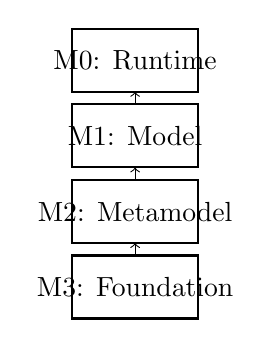
\begin{tikzpicture}[scale=0.8]
\draw[thick] (0,0) rectangle (2,1) node[midway] {M3: Foundation};
\draw[thick] (0,1.2) rectangle (2,2.2) node[midway] {M2: Metamodel};
\draw[thick] (0,2.4) rectangle (2,3.4) node[midway] {M1: Model};
\draw[thick] (0,3.6) rectangle (2,4.6) node[midway] {M0: Runtime};
\draw[->] (1,1) -- (1,1.2);
\draw[->] (1,2.2) -- (1,2.4);
\draw[->] (1,3.4) -- (1,3.6);
\end{tikzpicture}
\caption{MDE Pyramid: M3→M2→M1→M0 hierarchy with inter-level mappings}
\end{figure}

This hierarchy mirrors effective field theories at different energy scales, with effective logics at different abstraction levels.

\subsection{Convolution of Formal Systems}

\begin{definition}[Convolution of Formal Systems]
\label{def:convolution-formal}
We use a monoidal product $\star$ on logics with conservative projections. Large Language Models can be understood as convolutions of basic formal systems. Given a base formal system $\mathcal{L}_0$, the convolution creates extensions:
\[
\mathcal{L}_n = \mathcal{L}_0 \star \mathcal{L}_0 \star \cdots \star \mathcal{L}_0 \quad \text{(n times)}
\]
\end{definition}

\begin{theorem}[LLMs as Formal Language Models]
\label{thm:llm-formal}
Large Language Models are controllable extensions of convolutions of formal language models, where training learns the coupling constants that determine the effective theory.
\end{theorem}

\subsection{Hierarchy of Logics}

\begin{definition}[Hierarchy of Logics]
\label{def:hierarchy-logics}
The hierarchy: $\mathcal{L}_0 \subseteq \mathcal{L}_1 \subseteq \mathcal{L}_2 \subseteq \mathcal{L}_3$ where $\mathcal{L}_0$ is basic logic, $\mathcal{L}_1$ computational logic, $\mathcal{L}_2$ domain logic, and $\mathcal{L}_3$ application logic.
\end{definition}

\subsection{Inter-Level Mappings}

The mappings between levels are: M3→M2 (Gen4 primitive generates computational paradigms, see Section~\ref{sec:computation-paradigms}), M2→M1 (paradigms generate domain models via L/B/R structure, see Section~\ref{sec:formal-systems}), M1→M0 (domain models generate applications, see Sections~\ref{sec:boundary-maps}--\ref{sec:spectral-gap}).

\subsection{Derived Generating Functionals}

The logic includes derived operators providing higher-order structure:

\begin{definition}[Noe5: Noether's Theorem]
\label{def:noe5}
$\text{Noe5}: \text{Dir} \times B^4 \to B$ where $\text{Dir} = \{e_0, e_1, e_2, e_3\}$. Intuition: captures Noether's theorem \cite{noether1918} as invariance under ad$_i$ flow.
\end{definition}

\begin{definition}[CS5: Callan–Symanzik Stationarity]
\label{def:cs5}
$\text{CS5}: B^4 \times B \to B$ expressing RG stationarity. Intuition: captures stress-energy tensor with Callan–Symanzik equation as trace condition.
\end{definition}

\begin{definition}[Rice6: Rice's Theorem]
\label{def:rice6}
$\text{Rice6}(P[-], a, \mu): B$ where $P[-]$ is a term-context. Intuition: captures Rice's theorem \cite{rice1953} as impossibility of total positive discriminators for nontrivial projectors.
\end{definition}

Proofs and detailed constructions are given in Appendix~\ref{app:technical-derivations}.

\subsection{Domain Translation Architecture}

The logic provides universal structure; each domain provides semantic interpretation. Systematic mappings are documented in Table~\ref{tab:universal-domain-translation}. For detailed examples of Noether theorem and stress-energy tensor translations across domains, see Appendix~\ref{app:technical-derivations}.

The effective logic framework provides a unified structure for understanding how different computational paradigms emerge from the same underlying logical foundation. This framework translates systematically across domains as documented in Table~\ref{tab:universal-domain-translation}. In the next section, we will show how this framework reproduces and generalizes known theorems from logic, physics, and computation (Section~\ref{sec:consistency}), demonstrating the consistency of our approach with established results.
